\documentclass[titlepage]{article}
\usepackage{graphicx}
\usepackage{wrapfig}
\usepackage{enumitem}% http://ctan.org/pkg/enumitem
\graphicspath{ {./img/} }
\usepackage{listings}
\lstset{
  basicstyle=\small\ttfamily,
  columns=flexible,
  breaklines=true
}

\author{Jeffrey Meyer}
\title{Theory of Computer Sciece: Homework \#6 - NandToTetris | Assembly and Computer}

\begin{document}

\maketitle

\newpage

\section{Project 4}

\begin{description}
  \item[Mult]{\\

    \textbf{Mult.asm}

    \begin{lstlisting}
        // Initialize R2=0
        @2
        M=0
        // Initialize a=0
        @a
        M=0

      (LOOP)
        @a
        D=M
        @0
        D=D-M
        @HALT
        D;JGE // Check if a-r0 < 0

        @1
        D=M
        @2
        M=D+M
        @a
        M=M+1
        @LOOP
        0;JMP

      (HALT)
        @HALT
        0;JMP
    \end{lstlisting}

    All tests passed

    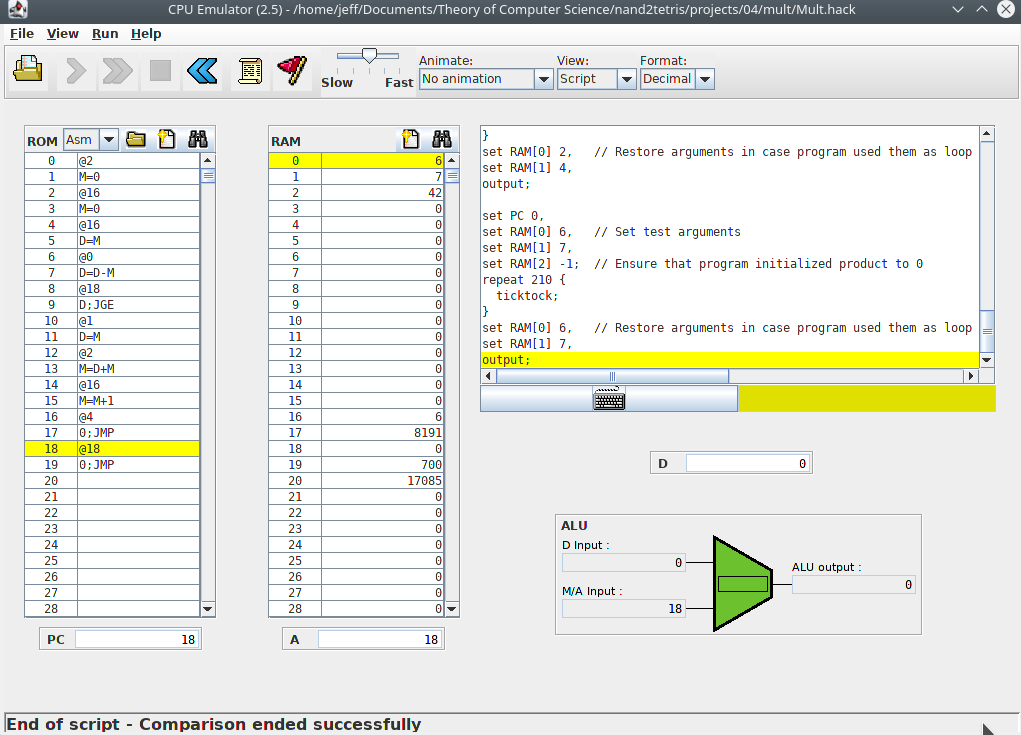
\includegraphics[width=.9\textwidth]{mult.png}
  }
  \item[Fill]{\\

    \textbf{Fill.asm}

    \begin{lstlisting}
        @SCREEN
        D=A
        @SCREEN_END
        M=D

        // Set screen length and screen end
        @8191
        D=A
        @SCREEN_LENGTH
        M=D
        @SCREEN_END
        M=M+D

        // set current position
        @SCREEN
        D=A


      (KEYCHECK)
        @KBD
        D=M
        // If key is pressed FILL_B if not FILL_W
        @FILL_B
        D;JGT
        @FILL_W
        0;JMP

      (FILL_B)
        @color
        M=-1
        @FILL
        0;JMP

      (FILL_W)
        @color
        M=0
        @FILL
        0;JMP

      (FILL)
        @SCREEN_LENGTH
        D=M
        @current
        M=D

        (NEXT)
          @current
          D=M
          @position
          M=D
          @SCREEN
          D=A
          @position
          M=M+D

          @color
          D=M
          @position
          A=M
          M=D

          @current
          D=M-1
          M=D

          @NEXT
          D;JGE

        @KEYCHECK

        0;JMP
    \end{lstlisting}

    Testing here was weird with the keypressing, so I took two screenshots. One before and one after pressing a key then pausing.

    First image is pressing $L$ while paused.

    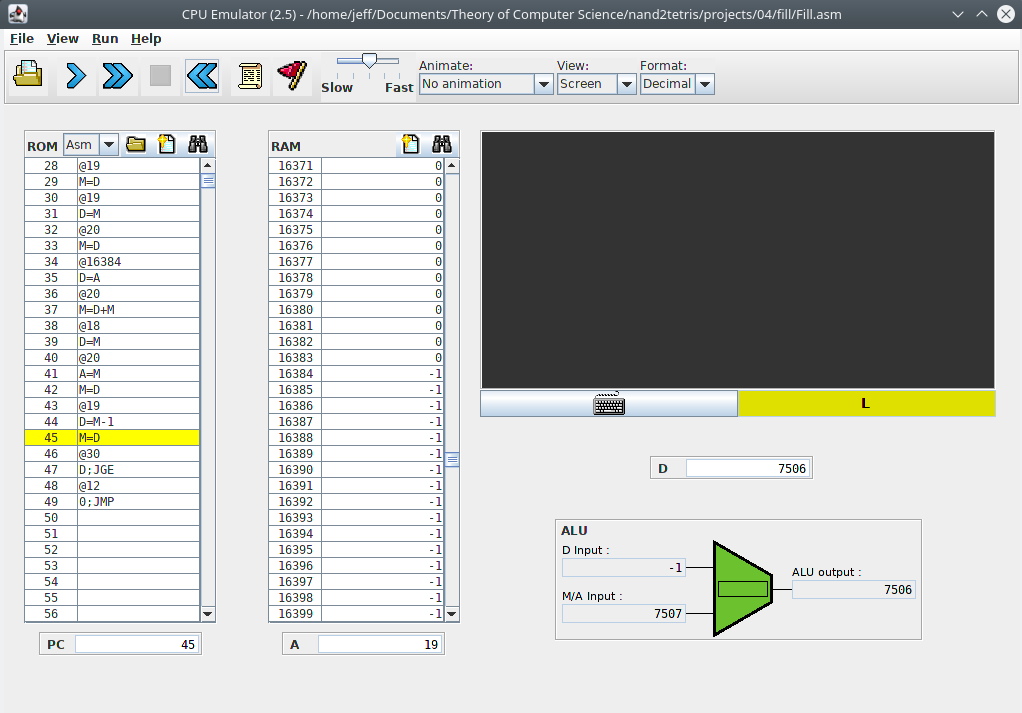
\includegraphics[width=.9\textwidth]{fill-0.png}

    The second image is after letting off of $L$ after unpausing.

    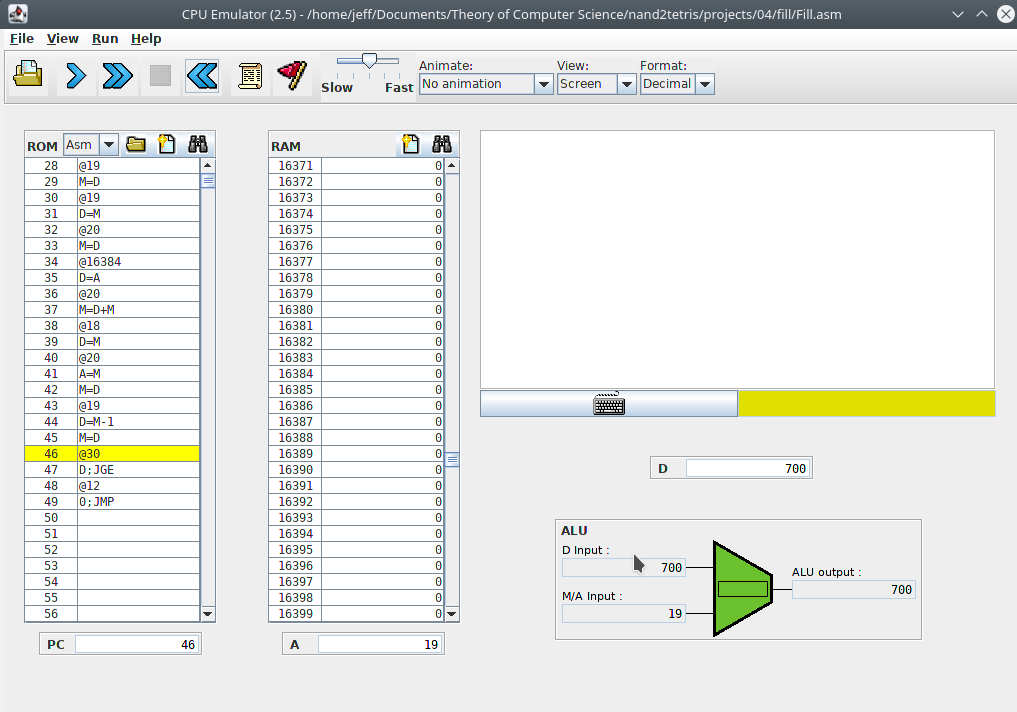
\includegraphics[width=.9\textwidth]{fill-1.png}
  }
\end{description}

\section{Project 5}

\begin{description}
  \item[Memory]{\\

    \textbf{Memory.hdl}

    \begin{lstlisting}
      CHIP Memory {
        IN in[16], load, address[15];
        OUT out[16];

        PARTS:
          // DMux on what part to load from
          DMux4Way(in=load, sel=address[13..14], a=loadA, b=loadB, c=loadC, d=loadD);
          // See if we need to load RAM normally or access keyboard or screen
          Or(a=loadA, b=loadB, out=loadRAM);
          // Define RAM
          RAM16K(in=in, load=loadRAM, address=address[0..13], out=outRAM);
          // Define Screen
          Screen(in=in, load=loadC, address=address[0..12], out=outScreen);
          // Define keyboard
          Keyboard(out=outKeyboard);
          // Output the output of the selected part
          Mux4Way16(sel=address[13..14], a=outRAM, b=outRAM, c=outScreen, d=outKeyboard, out=out);
      }
    \end{lstlisting}

    All tests passed.

    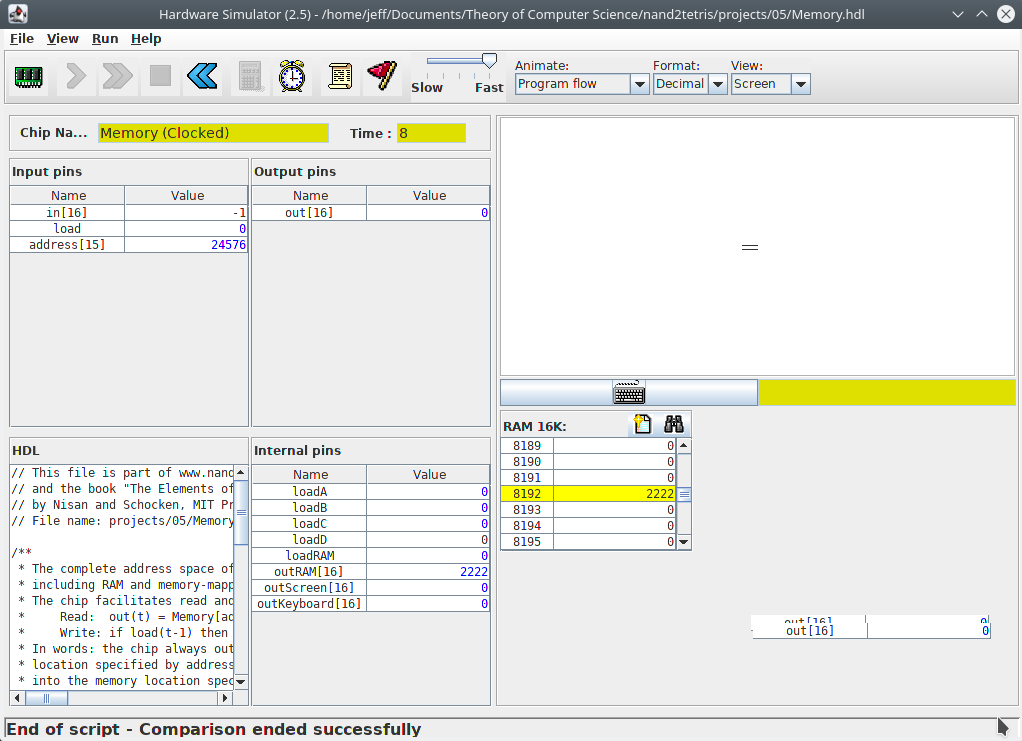
\includegraphics[width=.9\textwidth]{memory.png}
  }
  \item[CPU]{\\

    \textbf{CPU.hdl}

    \begin{lstlisting}
      CHIP CPU {
        IN inM[16],        // M value input  (M = contents of RAM[A])
          instruction[16], // Instruction for execution
          reset;           // Signals whether to re-start the current
                           // program (reset==1) or continue executing
                           // the current program (reset==0).

        OUT outM[16],      // M value output
          writeM,          // Write to M?
          addressM[15],    // Address in data memory (of M)
          pc[15];          // address of next instruction

        PARTS:
          // =============================================
          // Instruction Category
          // A = instruction[15] == 0
          // C = instruction[15] == 1

          // Calculate A or C instruction based on first bit
          Not(in=instruction[15], out=aInstruction);
          Not(in=aInstruction, out=cInstruction);


          // =============================================
          // Destinations
          // M = instruction[3]
          // D = instruction[4]
          // A = instruction[5]

          // Load A
          // loadAfromALU is based on if cInstruction and destination is the A register
          And(a=cInstruction, b=instruction[5], out=loadAfromALU);
          // loadA is based on if the ALU is loading it or the aInstruction is set
          Or(a=aInstruction, b=loadAfromALU, out=loadA);

          // Load D
          And(a=cInstruction, b=instruction[4], out=loadD);

          // Load M
          And(a=cInstruction, b=instruction[3], out=writeM);

          // A input
          Mux16(a=instruction, b=outALU, sel=loadAfromALU, out=inputA);


          // ==================================================
          // Operations
          // a-bit = instruction[12] // Whether to use Memory[A] or register A
          Mux16(a=registerA, b=inM, sel=instruction[12], out=AorM);


          // =============================================
          // Jumps
          Not(in=zr, out=nzr);
          Not(in=ng, out=nng);
          And(a=nzr, b=nng, out=pos);

          And(a=instruction[0], b=pos, out=jgt);
          And(a=instruction[1], b=zr, out=jeq);
          And8Way(in=true, in[0]=instruction[0], in[1]=instruction[1], in[2]=pos, out=jge);
          And(a=instruction[2], b=ng, out=jlt);
          And8Way(in=true, in[0]=instruction[0], in[1]=instruction[2], in[2]=nzr, out=jne);
          And8Way(in=true, in[0]=instruction[1], in[1]=instruction[2], in[2]=ng, out=jle);
          And8Way(in=true, in[0]=instruction[0], in[1]=instruction[1], in[2]=instruction[2], out=jmp);

          // If unconditional jump, less than or equal to, or greather than equal jump
          Or8Way(in=false, in[0]=jgt, in[1]=jeq, in[2]=jge, in[3]=jlt, in[4]=jne, in[5]=jle, in[6]=jmp, out=couldJump);
          And(a=cInstruction, b=couldJump, out=jump, out=loadPC);

          // =============================================
          // Define parts
          ARegister(in=inputA, load=loadA, out=registerA);
          DRegister(in=outALU, load=loadD, out=registerD);


          ALU(
            x=registerD,
            y=AorM,
            zx=instruction[11],
            nx=instruction[10],
            zy=instruction[9],
            ny=instruction[8],
            f=instruction[7],
            no=instruction[6],
            out=outALU,
            out=outM,
            zr=zr,
            ng=ng
          );

          // Finish Outputs
          Not(in=loadPC, out=incPC);
          PC(in=registerA, load=jump, inc=incPC, reset=reset, out[0..14]=pc);

          Or16(a=registerA, b=false, out[0..14]=addressM);
      }
    \end{lstlisting}

    \textbf{And8Way.hdl}

    \begin{lstlisting}
      CHIP And8Way {
        IN in[8];
        OUT out;

        PARTS:
          And(a=in[0], b=in[1], out=a);
          And(a=a, b=in[2], out=b);
          And(a=b, b=in[3], out=c);
          And(a=c, b=in[4], out=d);
          And(a=d, b=in[5], out=e);
          And(a=e, b=in[6], out=f);
          And(a=f, b=in[7], out=out);
      }
    \end{lstlisting}

    All tests passed.

    \textbf{CPU.tst}

    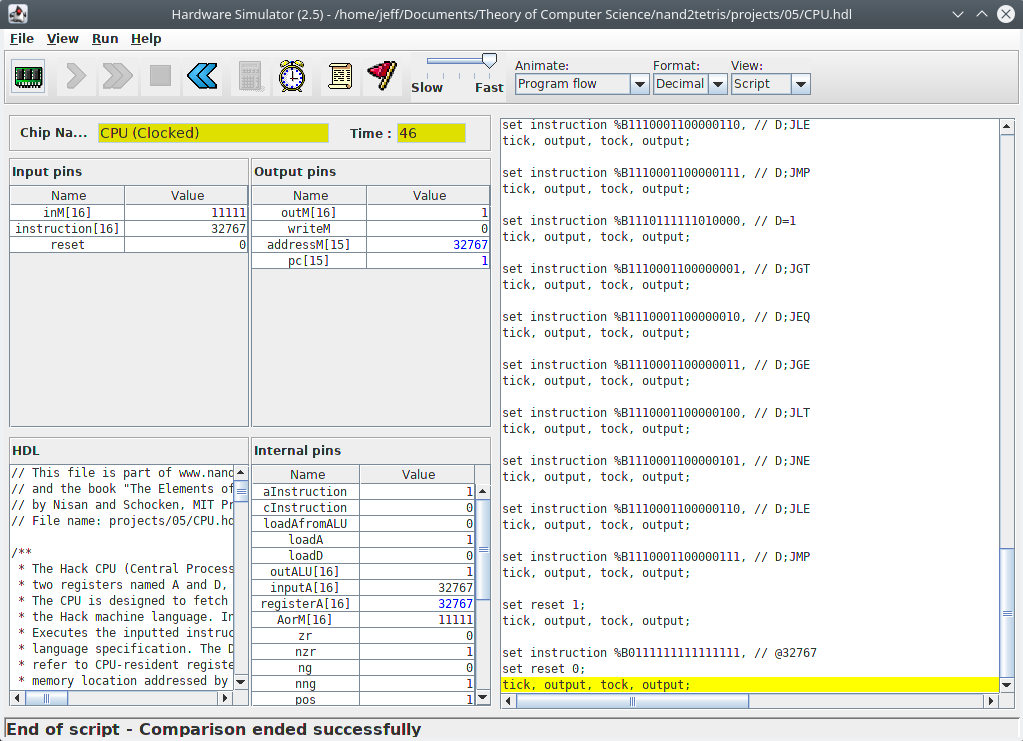
\includegraphics[width=.9\textwidth]{cpu.png}

    \textbf{CPU-External.tst}

    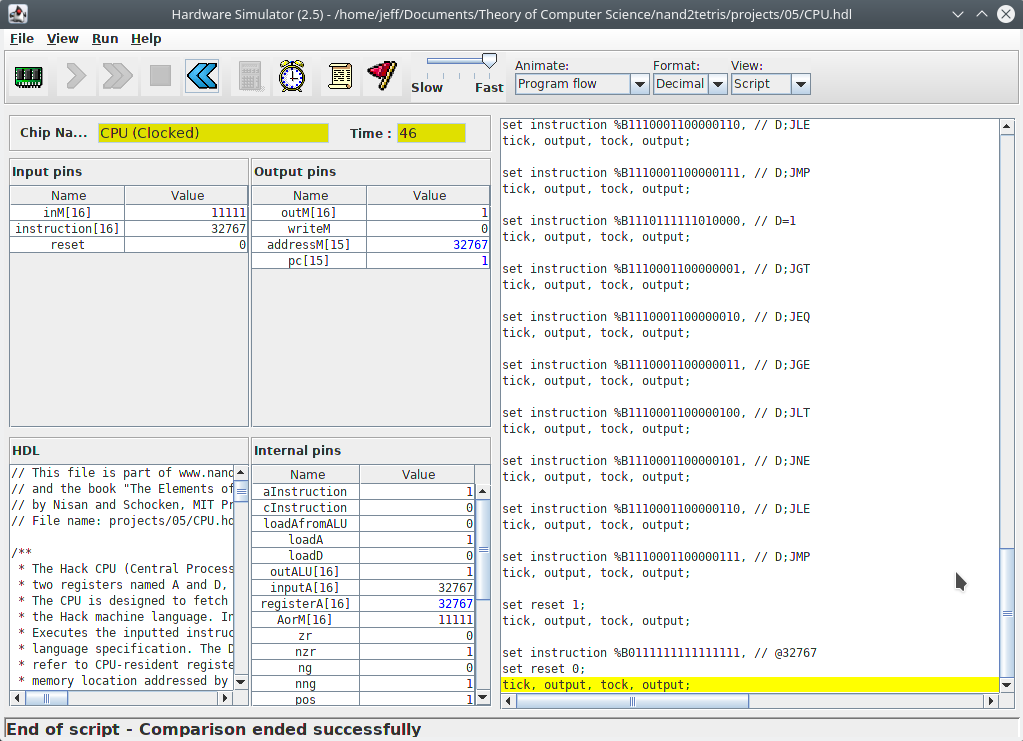
\includegraphics[width=.9\textwidth]{cpu-external.png}
  }
  \item[Computer]{\\

    \textbf{Computer.hdl}

    \begin{lstlisting}
      CHIP Computer {
        IN reset;

        PARTS:
          ROM32K(address=pc, out=instruction);
          CPU(inM=memory, instruction=instruction, reset=reset, outM=outM, writeM=writeM, addressM=addressM, pc=pc);
          Memory(in=outM, load=writeM, address=addressM, out=memory);
      }
    \end{lstlisting}

    \textbf{ComputerAdd.tst}

    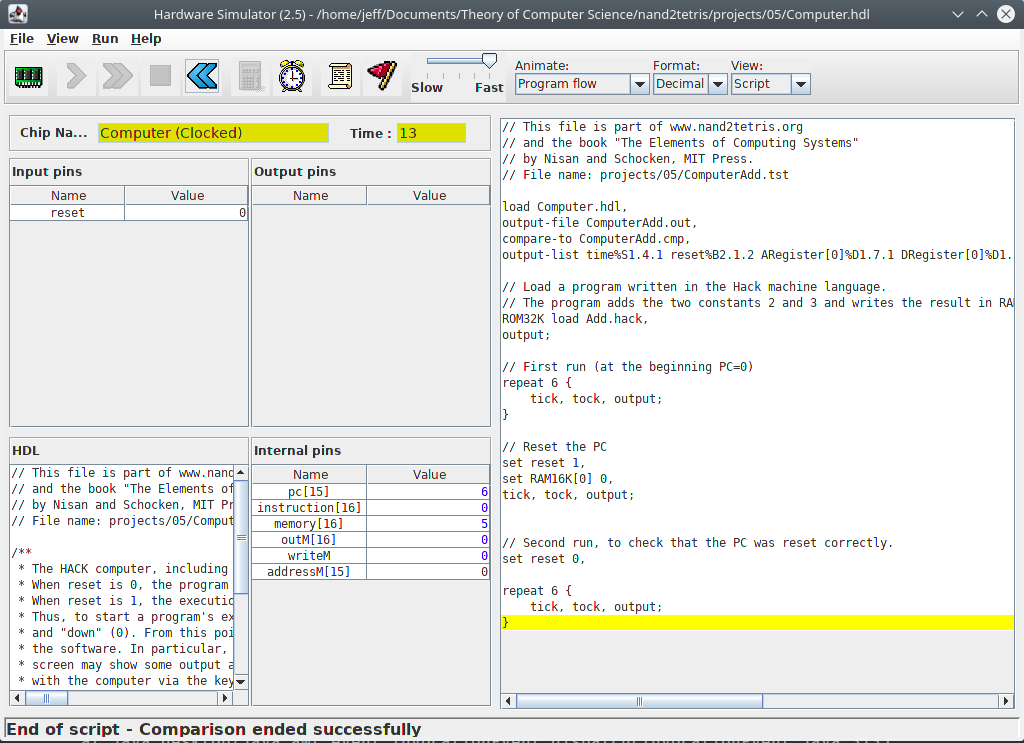
\includegraphics[width=.9\textwidth]{computer-add.png}

    \textbf{ComputerAdd-External.tst}

    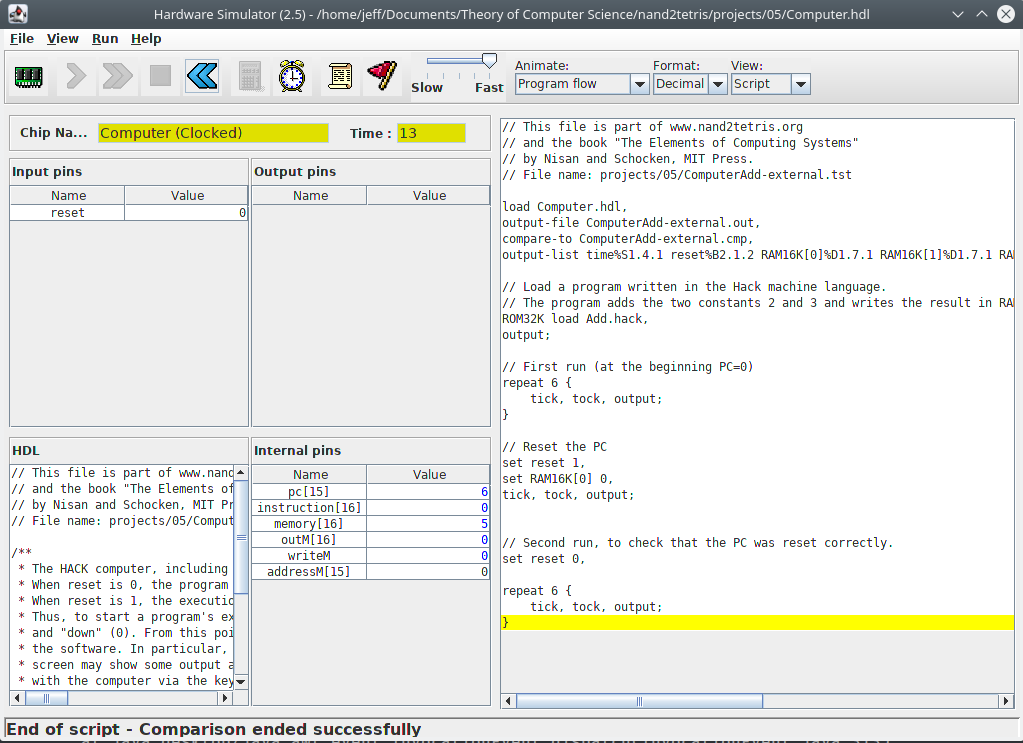
\includegraphics[width=.9\textwidth]{computer-add-external.png}

    \textbf{ComputerMax.tst}

    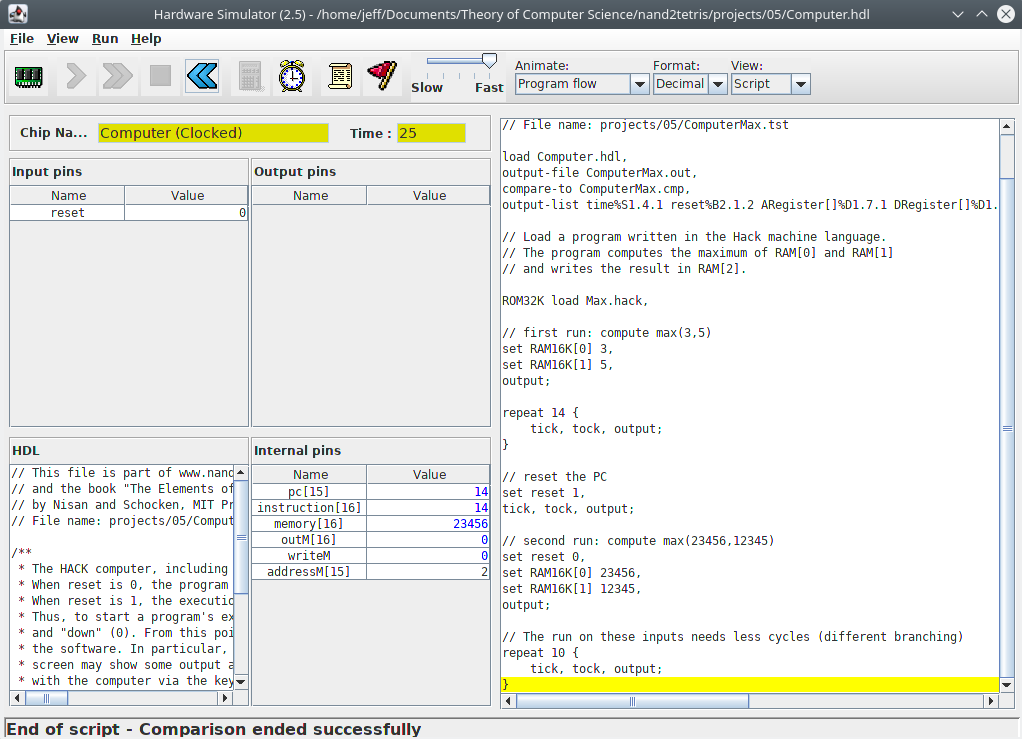
\includegraphics[width=.9\textwidth]{computer-max.png}

    \textbf{ComputerMax-External.tst}

    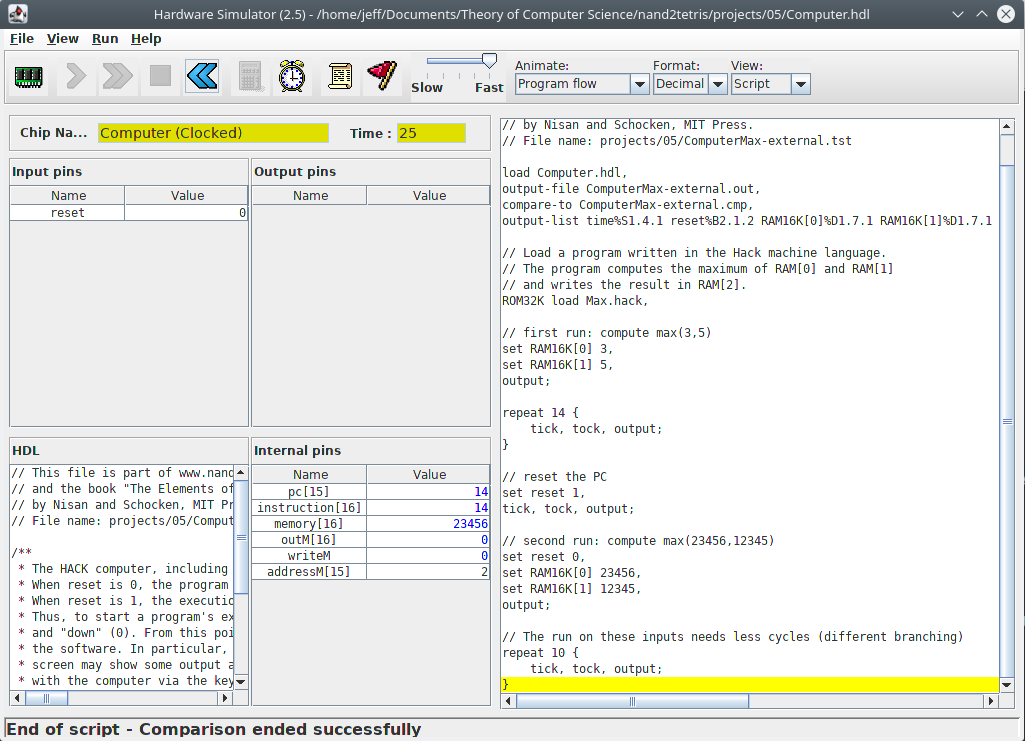
\includegraphics[width=.9\textwidth]{computer-max-external.png}

    \textbf{ComputerRect.tst}

    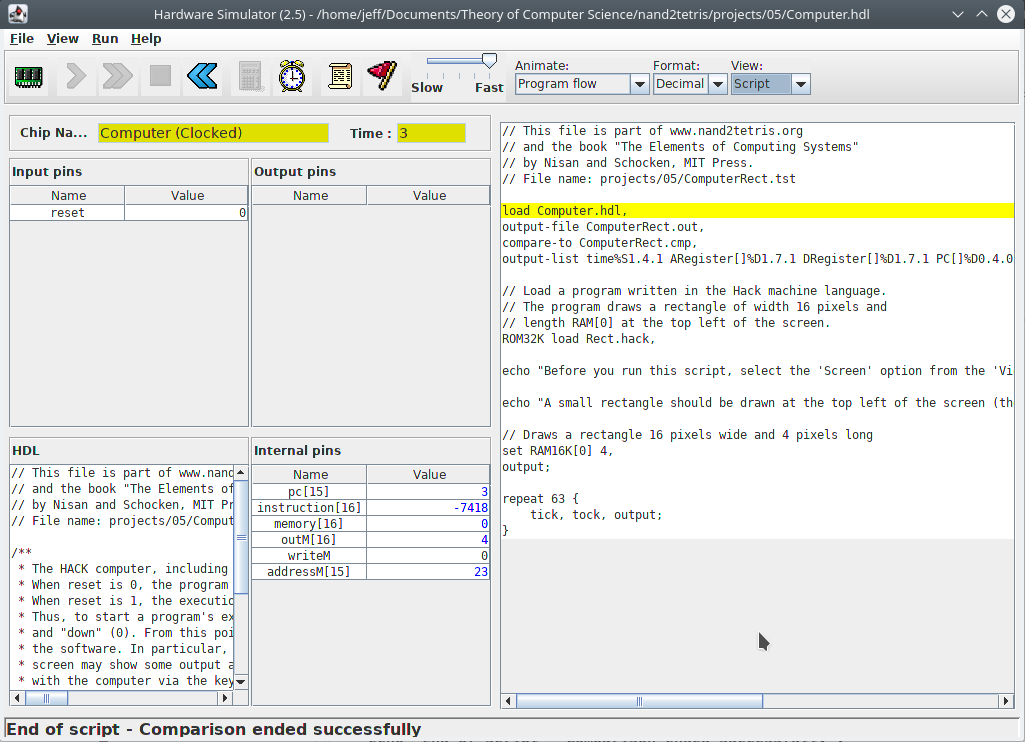
\includegraphics[width=.9\textwidth]{computer-rect.png}

    \textbf{ComputerRect-External.tst}

    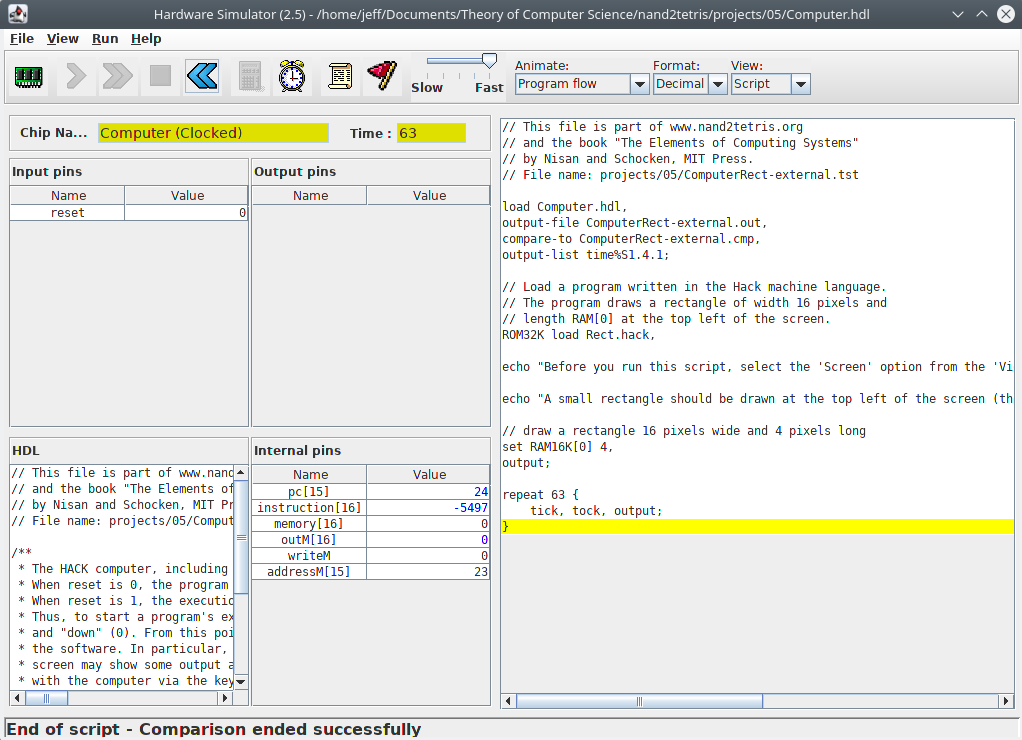
\includegraphics[width=.9\textwidth]{computer-rect-external.png}
  }
\end{description}

\end{document}